\documentclass[12pt,oneside]{article}
\usepackage{makeidx,anysize,mflogo,xspace,float,epsfig,url}
\usepackage{amsmath,amsfonts,amssymb,a4wide} 
\usepackage[utf8]{inputenc}
%\usepackage[francais]{babel}
%\usepackage[french]{babel}
\urlstyle{sf}
%\usepackage{subcaption}
\usepackage{hyperref}
\usepackage{graphicx}
\usepackage{graphics}
\usepackage{float}
\usepackage{caption}
\usepackage{colordvi} %??
\usepackage{listings} 
\usepackage{subfigure}
\usepackage{subfloat}
\usepackage{xcolor}
\graphicspath{{./figures/}}
%\usepackage[labelsep=quad,indention=10pt]{subfig}
\definecolor{grey}{rgb}{0.95,0.95,0.95} % on définit la couleur grise
	% (c'est un gris très clair)
	\definecolor{red}{rgb}{1.0,0.0,0.0} 
	\definecolor{green}{rgb}{0.0,1.0,0.0}
	\definecolor{blue}{rgb}{0.0,0.0,1.0}
	\lstloadlanguages{bash,Java,C,C++,csh,make,sh}%%[Visual]Basic,xml}
	\lstset{frame=none,basicstyle=\footnotesize,breaklines,tabsize=2,captionpos=b,
		prebreak={\hbox{$\rightarrow$}},postbreak={\hbox{$\hookrightarrow$}},
		showstringspaces=false,backgroundcolor=\color{grey}\bfseries,
		keywordstyle=\color{blue},commentstyle=\color{green}\textit,
		stringstyle=\color{red}\ttfamily,abovecaptionskip=2pt,aboveskip=0pt,
		belowskip=0pt,belowcaptionskip=0pt,numbers=none,columns=fullflexible, backgroundcolor=\color{grey}}
%left,numberstyle=\footnotesize,
%		stepnumber=2,numbersep=1pt}

\begin{document}


\begin{center}
{\bf \Large Redpitaya TCL programming} \\ \ \\
G. Goavec-M\'erou, J.-M Friedt \\ \ \\ \today
\end{center}

This tutorial is a sequel to the second one on which it is based. In addition to 
copying the ADC inputs to the DAC outputs, we wish (Fig. \ref{obj}) to {\bf mix} the stream of 
data coming from the ADC with a local numerically controlled oscillator ({\bf NCO}) and finally
filter ({\bf FIR}) before sending back to the DAC and the processing system
(Fig. \ref{fin}). In this tutorial, all such tasks will be achieved by programming in TCL rather than
using the graphical user interface of Vivado.

\begin{figure}[h!tb]
\begin{center}
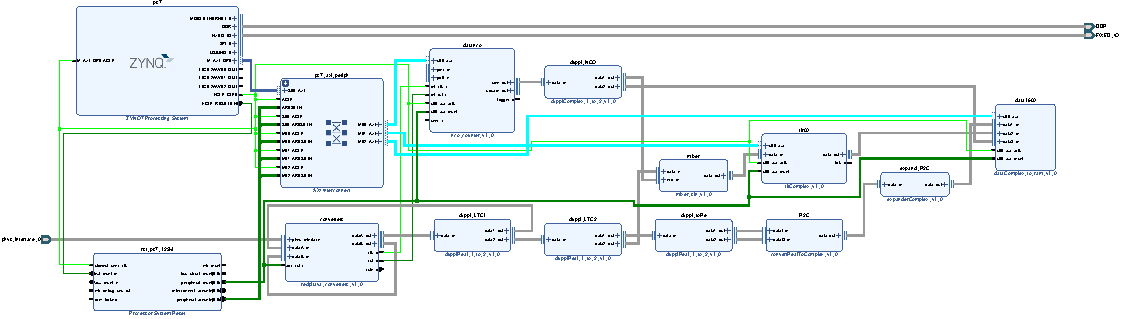
\includegraphics[width=\linewidth]{tutorial6}
\caption{Top: general objective of the frequency transposition of the input signal, followed by
filtering.}
\label{obj}
\end{center}

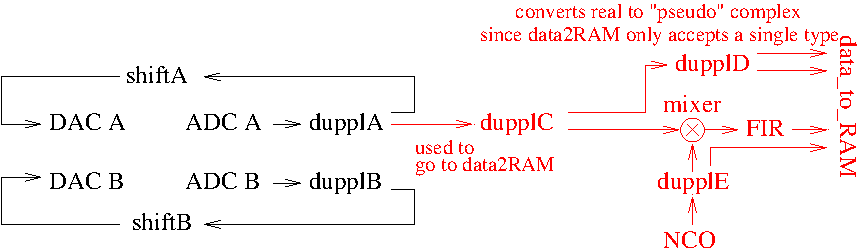
\includegraphics[width=\linewidth]{objective.pdf}
\caption{Schematic of the objective and final processing chain described in this document}
\label{fin}
\end{figure}

Starting from an existing TCL script, we first consider adding our processing blocks using the 
Vivado TCL commands as described at \url{https://www.xilinx.com/support/documentation/sw_manuals/xilinx2019_2/ug835-vivado-tcl-commands.pdf}.
The second part of the tutorial will wrap the Xilinx Vivado commands with custom OscimpDigital commands
to make the script compatible with the Altera/Intel synthesis tool.

\section{Initial TCL script}

Starting from {\tt tutorial3.tcl} in {\tt 3-PLPS/Design} which presents how to acquire data 
from the ADC and split the stream to send both the a data2ram and the DAC, we now wish to 
add the NCO + mixer + FIR filter.

The processor is instanciated:
{\footnotesize
\begin{verbatim}
startgroup
set ps7 [ create_bd_cell -type ip \
	-vlnv xilinx.com:ip:processing_system7:5.5 ps7 ]
set_property -dict [list CONFIG.PCW_IMPORT_BOARD_PRESET $board_preset ] $ps7
apply_bd_automation -rule xilinx.com:bd_rule:processing_system7 \
	-config {make_external "FIXED_IO, DDR" Master "Disable" Slave "Disable" } \
	$ps7
endgroup
\end{verbatim}
}

\noindent
followed by the ADC and DAC

{\footnotesize
\begin{verbatim}
set converters [ create_bd_cell -type ip -vlnv ggm:cogen:redpitaya_converters:1.0 converters]
set_property -dict [ list CONFIG.ADC_SIZE $ADC_SIZE \
	CONFIG.ADC_EN true \
	CONFIG.DAC_EN true] $converters
source $repo_path/redpitaya_converters/redpitaya_converters.tcl
connect_bd_intf_net [get_bd_intf_pins $converters/phys_interface] \
	[get_bd_intf_ports phys_interface_0]
\end{verbatim}
}

The streams are dupplicated to split between DAC and PS input

{\footnotesize
\begin{verbatim}
# dupplDataA
set dupplDataA [create_bd_cell -type ip -vlnv ggm:cogen:dupplReal_1_to_2:1.0 dupplDataA]
set_property -dict [ list CONFIG.DATA_SIZE $ADC_SIZE] $dupplDataA
connect_bd_intf_net [get_bd_intf_pins $converters/dataA_out] \
	[get_bd_intf_pins dupplDataA/data_in]

# dupplDataB
set dupplDataB [create_bd_cell -type ip -vlnv ggm:cogen:dupplReal_1_to_2:1.0 dupplDataB]
set_property -dict [ list CONFIG.DATA_SIZE $ADC_SIZE] $dupplDataB
connect_bd_intf_net [get_bd_intf_pins $converters/dataB_out] \
	[get_bd_intf_pins dupplDataB/data_in]
\end{verbatim}
}

Since in all Redpitayas the DAC is 14 bit but some Redpitayas are fitted with 16-bit ADC,
we shift to match bus sizes
{\footnotesize
\begin{verbatim}
# shifter is mandatory for redpitaya 16 : ADC is 16bits DAC 14bits
# shiftA_out
set shiftA_out [ create_bd_cell -type ip -vlnv ggm:cogen:shifterReal:1.0 shiftA_out]
set_property -dict [ list \
	CONFIG.SIGNED_FORMAT true \
	CONFIG.DATA_IN_SIZE $ADC_SIZE \
	CONFIG.DATA_OUT_SIZE 14] $shiftA_out
connect_bd_intf_net [get_bd_intf_pins dupplDataA/data2_out] \
	[get_bd_intf_pins $shiftA_out/data_in]
connect_bd_intf_net [get_bd_intf_pins shiftA_out/data_out] \
	[get_bd_intf_pins $converters/dataA_in]

# shiftB_out
set shiftB_out [ create_bd_cell -type ip -vlnv ggm:cogen:shifterReal:1.0 shiftB_out]
set_property -dict [ list \
	CONFIG.SIGNED_FORMAT true \
	CONFIG.DATA_IN_SIZE $ADC_SIZE \
	CONFIG.DATA_OUT_SIZE 14] $shiftB_out
connect_bd_intf_net [get_bd_intf_pins dupplDataB/data2_out] \
	[get_bd_intf_pins $shiftB_out/data_in]
connect_bd_intf_net [get_bd_intf_pins shiftB_out/data_out] \
	[get_bd_intf_pins $converters/dataB_in]
\end{verbatim}
}

Finally the data are sent to the PS
{\footnotesize
\begin{verbatim}
# convert realToComplex
set convertReal2Cplx [create_bd_cell -type ip -vlnv ggm:cogen:convertRealToComplex:1.0 convertReal2Cplx]
set_property -dict [ list CONFIG.DATA_SIZE $ADC_SIZE] $convertReal2Cplx
connect_bd_intf_net [get_bd_intf_pins dupplDataA/data1_out] \
	[get_bd_intf_pins convertReal2Cplx/dataI_in]
connect_bd_intf_net [get_bd_intf_pins dupplDataB/data1_out] \
	[get_bd_intf_pins convertReal2Cplx/dataQ_in]

# data2ram
set data1600 [create_bd_cell -type ip -vlnv ggm:cogen:dataComplex_to_ram:1.0 data1600]
set_property -dict [ list CONFIG.DATA_SIZE $ADC_SIZE \
						CONFIG.NB_INPUT {1} \
						CONFIG.NB_SAMPLE {4096}] $data1600
connect_bd_intf_net [get_bd_intf_pins convertReal2Cplx/data_out] \
	[get_bd_intf_pins data1600/data1_in]

apply_bd_automation -rule xilinx.com:bd_rule:axi4 \
    -config {Master "/ps7/M_AXI_GP0" Clk "Auto" } \
    [get_bd_intf_pins data1600/s00_axi]

connect_bd_net [get_bd_pins rst_ps7_125M/peripheral_reset] \
	[get_bd_pins $converters/adc_rst_i]
\end{verbatim}
}

The name of the interfaces are found using the {\tt oscimpDigital/fpga\_ip/tools/print\_businterfaces.py} and providing
as argument the directory name of the processing block in the {\tt fpga\_ip} directory. For example
{\tt ./tools/print\_businterfaces.py dupplComplex\_1\_to\_2}

{\footnotesize
\begin{verbatim}
./tools/print_businterfaces.py dupplComplex_1_to_2
component:
----------
name        : dupplComplex_1_to_2
VLNV        : ggm:cogen:dupplComplex_1_to_2:1.0
description : dupplComplex_1_to_2_v1_0

Parameters:
-----------
name: DATA_SIZE
  display name  : Data Size
    default value : 8
...
\end{verbatim}
}

\section{TCL script modifications}

The NCO AXI connection must be taken care of manually, following the same syntax as used in the data\_to\_ram block
with the apply\_bd\_automation command. Similarly, the NCO reset and clock must be connected to the converter clock
using 
{\footnotesize
\begin{verbatim}
connect_bd_net [get_bd_pins $converters/clk_o] \
	[get_bd_pins $datanco/ref_clk_i]
connect_bd_net [get_bd_pins $converters/rst_o] \
	[get_bd_pins $datanco/ref_rst_i]
\end{verbatim}
}
\noindent assuming the name of the NCO is {\tt datanco}.

See {\tt design/tutorial6.tcl} for the lines to be added to tutorial 2 to reach the expected result.

\end{document}

